\documentclass{csbeamer}

\usepackage{dsfont}
\usepackage{amsmath}
\usepackage{amssymb}
\usepackage{algorithm}
\usepackage{algpseudocode}

% Add custom color definitions for Dynamic Programming
\definecolor{dpmain}{HTML}{1565C0}
\definecolor{dpaccent}{HTML}{FF6B35}
\definecolor{dplight}{HTML}{42A5F5}
\definecolor{dpsecondary}{HTML}{4CAF50}
\definecolor{dpeval}{HTML}{9C27B0}
\definecolor{dpimprove}{HTML}{E91E63}
\definecolor{dpvalue}{HTML}{FF9800}
\definecolor{dppolicy}{HTML}{795548}

\university{St. Francis Xavier University}
\department{Department of Computer Science}
\course{CSCI-531 - Reinforcement Learning}
\courseshort{CSCI-531 - RL}
\term{Fall 2025}
\author{Dr. Jean-Alexis Delamer}

\title{Dynamic Programming}

\begin{document}

\frame{\titlepage}

% Section: Introduction
\section{Introduction}

\subsection{From Theory to Practice}

\begin{frame}
    \frametitle{From Theory to Practice: Computing Optimal Policies}

    \begin{block}<1->{What We Know So Far}
        \begin{itemize}
            \item<1-> How to model problems as \textcolor{dpmain}{\textbf{MDPs}}
            \item<2-> Why we need \textcolor{dpeval}{\textbf{policies}} and \textcolor{dpvalue}{\textbf{value functions}}
            \item<3-> What \textcolor{dpsecondary}{\textbf{optimal policies}} look like mathematically
        \end{itemize}
    \end{block}

    \begin{block}<4->{The Remaining Challenge}
        \begin{center}
            \large{\textcolor{dpaccent}{\textbf{How do we actually compute these optimal policies?}}}
        \end{center}
    \end{block}

    \begin{block}<5->{The Approach Menu}
        \begin{itemize}
            \item<5-> \textcolor{dpmain}{\textbf{Dynamic Programming}}: Complete knowledge of MDP
            \item<6-> \textcolor{dplight}{\textbf{Monte Carlo Methods}}: Learn from experience
            \item<7-> \textcolor{dpsecondary}{\textbf{Temporal Difference Learning}}: Combines both approaches
        \end{itemize}
    \end{block}
\end{frame}

\begin{frame}
    \frametitle{Why Start with Dynamic Programming?}

    \begin{columns}
        \begin{column}{0.6\textwidth}
            \begin{block}<1->{Three Key Reasons}
                \begin{enumerate}
                    \item<1-> \textcolor{dpmain}{\textbf{Conceptual Foundation}}
                        \begin{itemize}
                            \item Core principles used in all RL algorithms
                        \end{itemize}
                    \item<2-> \textcolor{dpaccent}{\textbf{Theoretical Clarity}}
                        \begin{itemize}
                            \item Shows exactly what we're trying to approximate
                        \end{itemize}
                    \item<3-> \textcolor{dpsecondary}{\textbf{Practical Utility}}
                        \begin{itemize}
                            \item Works perfectly when MDP is known
                        \end{itemize}
                \end{enumerate}
            \end{block}
        \end{column}

        \begin{column}{0.4\textwidth}
            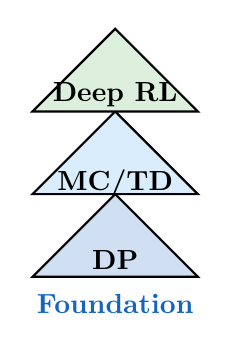
\begin{tikzpicture}[scale=0.7]
                \only<4->{
                    % Foundation pyramid
                    \draw[thick, fill=dpmain!20] (0,0) -- (3,0) -- (1.5,1.5) -- cycle;
                    \node at (1.5,0.3) {\textbf{DP}};

                    \draw[thick, fill=dplight!20] (0,1.5) -- (3,1.5) -- (1.5,3) -- cycle;
                    \node at (1.5,1.7) {\textbf{MC/TD}};

                    \draw[thick, fill=dpsecondary!20] (0,3) -- (3,3) -- (1.5,4.5) -- cycle;
                    \node at (1.5,3.3) {\textbf{Deep RL}};

                    \node at (1.5,-0.5) {\textcolor{dpmain}{\textbf{Foundation}}};
                }
            \end{tikzpicture}
        \end{column}
    \end{columns}

    \only<5->{
        \begin{center}
            \textcolor{dpaccent}{\textbf{What do we need to calculate to obtain optimal policies?}}
        \end{center}
    }
\end{frame}

% Section: Policy Iteration
\section{Policy Iteration}

\subsection{The Intuitive Approach}

\begin{frame}
    \frametitle{Policy Iteration: The Intuitive Approach}

    \begin{block}<1->{Core Idea}
        Start with any policy, then repeatedly improve it until optimal
    \end{block}

    \begin{block}<2->{Two Alternating Steps}
        \begin{enumerate}
            \item<2-> \textcolor{dpeval}{\textbf{Policy Evaluation}}: How good is current policy?
            \item<3-> \textcolor{dpimprove}{\textbf{Policy Improvement}}: Update policy based on values
        \end{enumerate}
    \end{block}

    \begin{center}
        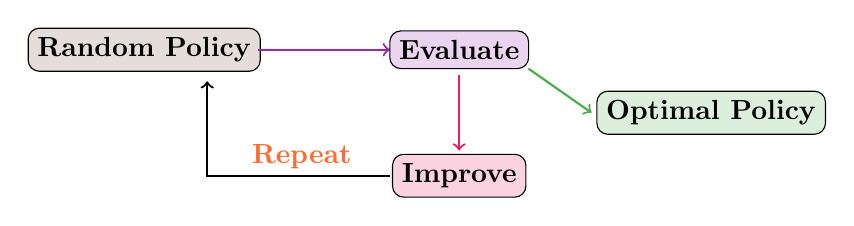
\begin{tikzpicture}[scale=0.8]
            \only<4->{
                % Flow diagram
                \node[draw, rounded corners, fill=dppolicy!20] at (0,2) {\textbf{Random Policy}};

                \draw[->, thick, dpeval] (1.8,2) -- (3.9,2);
                \node[draw, rounded corners, fill=dpeval!20] at (5,2) {\textbf{Evaluate}};

                \draw[->, thick, dpimprove] (5,1.6) -- (5,0.4);
                \node[draw, rounded corners, fill=dpimprove!20] at (5,0) {\textbf{Improve}};

                \draw[->, thick] (3.9,0) -- (1,0) -- (1,1.5);

                \node at (2.5,0.3) {\textcolor{dpaccent}{\textbf{Repeat}}};

                \node[draw, rounded corners, fill=dpsecondary!20] at (9,1) {\textbf{Optimal Policy}};
                \draw[->, thick, dpsecondary] (6.1,1.7) -- (7.1,1);
            }
        \end{tikzpicture}
    \end{center}

    \only<5->{
        \begin{center}
            \textcolor{dpmain}{\textbf{Each improvement step makes the policy better (or keeps it optimal)}}
        \end{center}
    }
\end{frame}

\subsection{Policy Evaluation}

\begin{frame}
    \frametitle{Policy Evaluation: Computing Value Functions}

    \begin{block}<1->{The Challenge}
        Given policy $\pi$, compute $v_\pi(s)$ for all states using:
        \begin{equation*}
            v_\pi(s) = \sum_a\pi(a|s)\sum_{s'}p(s'|s,a)\left[ r(s,a) + \gamma v_\pi(s') \right]
        \end{equation*}
    \end{block}

    \begin{block}<2->{The Problem}
        \begin{itemize}
            \item<2-> This equation is \textcolor{dpaccent}{\textbf{circular}}!
            \item<3-> Value of state $s$ depends on values of future states $s'$
            \item<4-> We have a system of $|S|$ equations with $|S|$ unknowns
        \end{itemize}
    \end{block}
\end{frame}

\begin{frame}
    \frametitle{Policy Evaluation: Computing Value Functions}

    \begin{block}<1->{The Challenge}
        Given policy $\pi$, compute $v_\pi(s)$ for all states using:
        \begin{equation*}
            v_\pi(s) = \sum_a\pi(a|s)\sum_{s'}p(s'|s,a)\left[ r(s,a) + \gamma v_\pi(s') \right]
        \end{equation*}
    \end{block}

    \begin{block}<2->{The Solution: Iterative Approximation}
        \begin{enumerate}
            \item<2-> Start with initial guesses $v_0(s)$ (often zeros)
            \item<3-> Iteratively improve estimates using Bellman equation
            \item<4-> Continue until values stabilize
        \end{enumerate}
    \end{block}
\end{frame}

\begin{frame}
    \frametitle{Policy Evaluation Algorithm}

    \begin{algorithm}[H]
    \caption{Policy Evaluation}
    \begin{algorithmic}[1]
    \State \textbf{Initialize:} $V(s) \in \mathbb{R}$ arbitrarily, $V(\text{terminal}) = 0$
    \Repeat
        \State $\Delta \leftarrow 0$
        \For{each state $s$}
            \State $v \leftarrow V(s)$
            \State $V(s) \leftarrow \sum_a\pi(a|s)\sum_{s'}p(s'|s,a)[r + \gamma V(s')]$
            \State $\Delta \leftarrow \max(\Delta, |v - V(s)|)$
        \EndFor
    \Until{$\Delta < \theta$ (small threshold)}
    \end{algorithmic}
    \end{algorithm}
\end{frame}

\begin{frame}
    \frametitle{Policy Evaluation: Intuition}

    \begin{center}
        \begin{tikzpicture}[scale=1.0]
            % Grid world example
            \only<1->{
                % Grid with better styling
                \draw[step=1.5cm,gray!40,thick] (0,0) grid (6,4.5);

                % Add coordinate labels
                \foreach \x in {0,1,2,3} {
                    \node[gray] at (\x*1.5+0.4,4.3) {(\x,2)};
                    \node[gray] at (\x*1.5+0.4,2.8) {(\x,1)};
                    \node[gray] at (\x*1.5+0.4,1.3) {(\x,0)};
                }

                % States with initial values - improved styling
                \foreach \x in {0,1,2,3} {
                    \foreach \y in {0,1,2} {
                        \draw[fill=dplight!20,draw=dpmain,thick] (\x*1.5+0.75,\y*1.5+0.75) circle (0.35);
                        \node at (\x*1.5+0.75,\y*1.5+0.75) {\small\textbf{0.0}};
                    }
                }

                % Goal state
                \draw[fill=dpsecondary!70,draw=dpsecondary,very thick] (5.25,3.75) circle (0.35);
                \node at (5.25,3.75) {\small\textbf{+1}};
                \node[dpsecondary,below] at (5.25,3.4) {\tiny\textbf{GOAL}};

                % Policy arrows
                \draw[->, very thick, dppolicy] (1.1,0.75) -- (1.9,0.75);
                \draw[->, very thick, dppolicy] (2.6,0.75) -- (3.4,0.75);
                \draw[->, very thick, dppolicy] (4.1,0.75) -- (4.9,0.75);
                \draw[->, very thick, dppolicy] (5.25,1.1) -- (5.25,1.9);

                \draw[->, very thick, dppolicy] (1.1,2.25) -- (1.9,2.25);
                \draw[->, very thick, dppolicy] (2.6,2.25) -- (3.4,2.25);
                \draw[->, very thick, dppolicy] (3.75,2.6) -- (3.75,3.4);
                \draw[->, very thick, dppolicy] (5.25,2.6) -- (5.25,3.4);

                \draw[->, very thick, dppolicy] (1.1,3.75) -- (1.9,3.75);
                \draw[->, very thick, dppolicy] (2.6,3.75) -- (3.4,3.75);
                \draw[->, very thick, dppolicy] (4.1,3.75) -- (4.9,3.75);

                % Policy legend
                \draw[->, very thick, dppolicy] (6.5,3.5) -- (7.0,3.5);
                \node[right] at (7.1,3.5) {\small Policy $\pi$};

                \node at (2,-0.5) {\large\textcolor{dpmain}{\textbf{Iteration 0: Initialize all values to 0}}};
            }

            \only<2->{
                % After iteration 1 - show immediate neighbors
                \draw[fill=dpeval!30,draw=dpeval,thick] (3.75,3.75) circle (0.35);
                \node at (3.75,3.75) {\small\textbf{0.9}};

                \draw[fill=dpeval!30,draw=dpeval,thick] (5.25,2.25) circle (0.35);
                \node at (5.25,2.25) {\small\textbf{0.9}};

                % Highlight the value flow with arrows
                \draw[->, dpeval, very thick, dashed] (5.25,3.4) -- (5.25,2.6);
                \draw[->, dpeval, very thick, dashed] (4.9,3.75) -- (4.1,3.75);

                \node[dpeval] at (7.1,3) {$\gamma = 0.9$};

                \node at (2,-1) {\large\textcolor{dpeval}{\textbf{Iteration 1: Values propagate to immediate neighbors}}};
            }

            \only<3->{
                % After iteration 2 - show further propagation
                \draw[fill=dpvalue!40,draw=dpvalue,thick] (2.25,3.75) circle (0.35);
                \node at (2.25,3.75) {\small\textbf{0.81}};

                \draw[fill=dpvalue!40,draw=dpvalue,thick] (3.75,2.25) circle (0.35);
                \node at (3.75,2.25) {\small\textbf{0.81}};

                \draw[fill=dpvalue!40,draw=dpvalue,thick] (5.25,0.75) circle (0.35);
                \node at (5.25,0.75) {\small\textbf{0.73}};

                % Show discount factor effect
                \node[dpvalue] at (7.1,2.5) {$\gamma = 0.9$};

                \node at (2,-1.5) {\large\textcolor{dpvalue}{\textbf{Iteration 2: Values continue propagating (discounted)}}};
            }

            \only<4->{
                % Final convergence - show all updated values
                \draw[fill=dpaccent!50,draw=dpaccent,thick] (2.25,2.25) circle (0.35);
                \node at (2.25,2.25) {\small\textbf{0.66}};

                \draw[fill=dpaccent!50,draw=dpaccent,thick] (0.75,3.75) circle (0.35);
                \node at (0.75,3.75) {\small\textbf{0.59}};

                \draw[fill=dpaccent!50,draw=dpaccent,thick] (3.75,0.75) circle (0.35);
                \node at (3.75,0.75) {\small\textbf{0.59}};

                % Add convergence indicator
                \node[dpaccent] at (7.1,2) {Converged};

                \node at (2,-2) {\large\textcolor{dpaccent}{\textbf{Convergence: Optimal values for given policy}}};
            }
        \end{tikzpicture}
    \end{center}
\end{frame}

\subsection{Policy Improvement}

\begin{frame}
    \frametitle{Policy Improvement: Making Better Decisions}

    \begin{block}<1->{The Question}
        Given policy $\pi$ and its value function $v_\pi$, can we find a better policy?
    \end{block}

    \begin{block}<2->{The Approach: Be Greedy!}
        For each state $s$, examine all possible actions:
        \begin{equation*}
            q_\pi(s,a) = \sum_{s'}p(s'|s,a)\left[r(s,a) + \gamma v_\pi(s')\right]
        \end{equation*}

        \textit{"What happens if I take action $a$ in state $s$, then follow policy $\pi$?"}
    \end{block}

    \begin{block}<3->{Improved Policy}
        Create new policy $\pi'$ by being greedy:
        \begin{equation*}
            \pi'(s) = \arg\max_a q_\pi(s,a) = \arg\max_a \sum_{s'}p(s'|s,a)\left[r(s,a) + \gamma v_\pi(s')\right]
        \end{equation*}
    \end{block}
\end{frame}

\begin{frame}
    \frametitle{Policy Improvement Theorem}

    \begin{block}<1->{Theorem}
        If $\pi$ and $\pi'$ are policies such that for all $s \in S$:
        \begin{equation*}
            q_\pi(s,\pi'(s)) \geq v_\pi(s)
        \end{equation*}

        Then policy $\pi'$ must be as good as or better than $\pi$:
        \begin{equation*}
            v_{\pi'}(s) \geq v_\pi(s) \text{ for all } s \in S
        \end{equation*}
    \end{block}

    \begin{block}<2->{Intuition}
        \begin{itemize}
            \item<2-> \textcolor{dpmain}{\textbf{Acting optimally for one step, then following old policy}}
            \item<3-> Can only make things \textcolor{dpsecondary}{\textbf{better}} (or stay the same)        \end{itemize}
    \end{block}

    \only<4->{
        \begin{center}
            \textcolor{dpaccent}{\textbf{Guaranteed improvement or stability!}}
        \end{center}
    }
\end{frame}

\subsection{Complete Policy Iteration Algorithm}

\begin{frame}
    \frametitle{Policy Iteration Algorithm}

    \begin{block}<1->{Complete Process}
        \begin{enumerate}
            \item<1-> \textbf{Initialize}: Start with arbitrary policy $\pi_0$
            \item<2-> \textcolor{dpeval}{\textbf{Policy Evaluation}}: Compute $v_\pi$ for current policy
            \item<3-> \textcolor{dpimprove}{\textbf{Policy Improvement}}: Compute improved policy $\pi'$ from $v_\pi$
            \item<4-> \textbf{Check}: If $\pi' = \pi$, STOP (found $\pi^*$)
            \item<5-> \textbf{Otherwise}: Set $\pi = \pi'$ and go to step 2
        \end{enumerate}
    \end{block}

    \begin{block}<6->{Convergence Guarantee}
        \begin{itemize}
            \item<6-> MDPs have finite number of deterministic policies
            \item<7-> Each improvement makes policy strictly better (unless optimal)
            \item<8-> \textcolor{dpsecondary}{\textbf{Must converge to optimal policy in finite steps}}
        \end{itemize}
    \end{block}
\end{frame}

\begin{frame}
    \frametitle{Policy Iteration Example}

    \begin{center}
        \begin{tikzpicture}[scale=0.8]
            % Show progression through iterations with clear 3x2 gridworld
            \only<1->{
                % Step 1: Initial Random Policy
                \node at (1.5,4.5) {\textcolor{dppolicy}{\textbf{Step 1: Random Policy}}};

                % Grid
                \draw[step=1cm,gray!40,thick] (0,2) grid (3,4);

                % States with random policy arrows
                \foreach \x/\y in {0.5/3.5, 1.5/3.5, 2.5/3.5, 0.5/2.5, 1.5/2.5} {
                    \draw[fill=dplight!20,draw=dpmain] (\x,\y) circle (0.25);
                }

                % Goal state
                \draw[fill=dpsecondary!70,draw=dpsecondary,very thick] (2.5,2.5) circle (0.25);

                % Random policy arrows
                \draw[->, very thick, dppolicy] (0.5,3.2) -- (0.5,2.8); % down
                \draw[->, very thick, dppolicy] (1.8,3.3) -- (2.2,3.3); % right
                \draw[->, very thick, dppolicy] (2.2,3.7) -- (1.8,3.7); % left
                \draw[->, very thick, dppolicy] (0.8,2.5) -- (1.2,2.5); % right
                \draw[->, very thick, dppolicy] (1.5,2.8) -- (1.5,3.2); % up

                \node at (1.5,1.5) {\small\textcolor{dppolicy}{\textbf{Random actions}}};
            }

            \only<2->{
                % Step 2: Policy Evaluation
                \node at (6.5,4.5) {\textcolor{dpeval}{\textbf{Step 2: Evaluate}}};

                % Grid with same structure
                \draw[step=1cm,gray!40,thick] (5,2) grid (8,4);

                % States with values
                \draw[fill=dpeval!30,draw=dpeval,thick] (5.5,3.5) circle (0.25);
                \node at (5.5,3.5) {\tiny\textbf{0.4}};

                \draw[fill=dpeval!30,draw=dpeval,thick] (6.5,3.5) circle (0.25);
                \node at (6.5,3.5) {\tiny\textbf{0.7}};

                \draw[fill=dpeval!30,draw=dpeval,thick] (7.5,3.5) circle (0.25);
                \node at (7.5,3.5) {\tiny\textbf{0.6}};

                \draw[fill=dpeval!30,draw=dpeval,thick] (5.5,2.5) circle (0.25);
                \node at (5.5,2.5) {\tiny\textbf{0.8}};

                \draw[fill=dpeval!30,draw=dpeval,thick] (6.5,2.5) circle (0.25);
                \node at (6.5,2.5) {\tiny\textbf{0.9}};

                % Goal state
                \draw[fill=dpsecondary!70,draw=dpsecondary,very thick] (7.5,2.5) circle (0.25);
                \node at (7.5,2.5) {\tiny\textbf{1.0}};

                \node at (6.5,1.5) {\small\textcolor{dpeval}{\textbf{Computed values}}};
            }

            \only<3->{
                % Step 3: Policy Improvement
                \node at (11.5,4.5) {\textcolor{dpimprove}{\textbf{Step 3: Improve}}};

                % Grid with same structure
                \draw[step=1cm,gray!40,thick] (10,2) grid (13,4);

                % States with improved policy arrows
                \foreach \x/\y in {10.5/3.5, 11.5/3.5, 12.5/3.5, 10.5/2.5, 11.5/2.5} {
                    \draw[fill=dpimprove!30,draw=dpimprove] (\x,\y) circle (0.25);
                }

                % Goal state
                \draw[fill=dpsecondary!70,draw=dpsecondary,very thick] (12.5,2.5) circle (0.25);

                % Greedy policy arrows (toward highest values)
                \draw[->, very thick, dpimprove] (10.8,2.5) -- (11.2,2.5); % right (0.8 > others)
                \draw[->, very thick, dpimprove] (11.8,2.5) -- (12.2,2.5); % right (goal adjacent)
                \draw[->, very thick, dpimprove] (11.5,3.2) -- (11.5,2.8); % down (goal adjacent)
                \draw[->, very thick, dpimprove] (10.8,3.5) -- (11.2,3.5); % right (toward 0.9)
                \draw[->, very thick, dpimprove] (12.5,3.2) -- (12.5,2.8); % down (toward goal)

                \node at (11.5,1.5) {\small\textcolor{dpimprove}{\textbf{Greedy actions}}};
            }
        \end{tikzpicture}
    \end{center}

    \begin{block}<4->{Key Insight}
        \textcolor{dpmain}{\textbf{Each iteration makes the policy strictly better until optimal}}
    \end{block}
\end{frame}

% Section: Value Iteration
\section{Value Iteration}

\subsection{A More Efficient Approach}

\begin{frame}
    \frametitle{Value Iteration: Cutting the Bottleneck}

    \begin{block}<1->{Policy Iteration's Bottleneck}
        \begin{itemize}
            \item<1-> Full policy evaluation requires multiple sweeps through all states
            \item<2-> Each evaluation step can be \textcolor{dpaccent}{\textbf{computationally expensive}}
            \item<3-> We do complete evaluation before any improvement
        \end{itemize}
    \end{block}

    \begin{block}<4->{Value Iteration's Insight}
        \textcolor{dpmain}{\textbf{What if we combine evaluation and improvement?}}
        \begin{itemize}
            \item<5-> Don't need full evaluation before improving
            \item<6-> One step of evaluation gives useful information
            \item<7-> Always act greedily based on current value estimates
        \end{itemize}
    \end{block}

    \only<8->{
        \begin{center}
            \textcolor{dpsecondary}{\textbf{Skip the separate policy - work directly with values!}}
        \end{center}
    }
\end{frame}

\begin{frame}
    \frametitle{Value Iteration Formula}

    \begin{block}<1->{Key Difference}
        Instead of following a fixed policy, always choose the best action:
        \begin{equation*}
            v_{k+1}(s) = \max_a\sum_{s'}p(s'|s,a)\left[ r(s,a) + \gamma v_k(s') \right]
        \end{equation*}
        \end{block}

    \begin{block}<2->{Comparison}
        \textbf{Policy Iteration says}:
        \begin{itemize}
            \item<2-> "Fully evaluate my current strategy, then improve it"
        \end{itemize}

        \textbf{Value Iteration says}:
        \begin{itemize}
            \item<3-> "Always act greedily based on current value estimates"
        \end{itemize}
    \end{block}
\end{frame}


\begin{frame}
    \frametitle{Value Iteration Formula}

    \begin{block}<1->{Key Difference}
        Instead of following a fixed policy, always choose the best action:
        \begin{equation*}
            v_{k+1}(s) = \max_a\sum_{s'}p(s'|s,a)\left[ r(s,a) + \gamma v_k(s') \right]
        \end{equation*}
        \end{block}

    \begin{block}<2->{Connection to Bellman Optimality}
        This directly solves the Bellman optimality equation:
        \begin{equation*}
            v^*(s) = \max_a\sum_{s'}p(s'|s,a)\left[ r(s,a) + \gamma v^*(s') \right]
        \end{equation*}
    \end{block}
\end{frame}

\begin{frame}
    \frametitle{Value Iteration Algorithm}

    \begin{block}<1->{Value Iteration Algorithm}
        \begin{enumerate}
            \item<1-> \textbf{Initialize}: $V(s) \in \mathbb{R}$ arbitrarily for all $s \in S$, $V(\text{terminal}) = 0$
            \item<2-> \textbf{Repeat} until convergence:
            \begin{itemize}
                \item<2-> $\Delta \leftarrow 0$
                \item<3-> \textbf{For} each state $s \in S$:
                \begin{itemize}
                    \item<3-> $v \leftarrow V(s)$
                    \item<4-> $V(s) \leftarrow \max_a \sum_{s'}p(s'|s,a)[r + \gamma V(s')]$
                    \item<5-> $\Delta \leftarrow \max(\Delta, |v - V(s)|)$
                \end{itemize}
            \end{itemize}
            \item<6-> \textbf{Until} $\Delta < \theta$ (convergence threshold)
            \item<7-> \textbf{Extract policy}: $\pi(s) = \arg\max_a\sum_{s'}p(s'|s,a)[r + \gamma V(s')]$
        \end{enumerate}
    \end{block}

    \begin{block}<8->{Key Advantages}
        \begin{itemize}
            \item<8-> \textcolor{dpsecondary}{\textbf{Simpler}}: No separate policy evaluation phase
            \item<9-> \textcolor{dpaccent}{\textbf{More efficient}}: Often faster per iteration
        \end{itemize}
    \end{block}
\end{frame}

\begin{frame}
    \frametitle{Value Iteration vs Policy Iteration}

    \begin{center}
        \begin{tabular}{|l|c|c|}
        \hline
        \textbf{Aspect} & \textbf{Policy Iteration} & \textbf{Value Iteration} \\
        \hline
        \textbf{Approach} & Evaluate then improve & Combined eval+improve \\
        \hline
        \textbf{Per iteration} & Slower (full eval) & Faster (one step) \\
        \hline
        \textbf{Total iterations} & Fewer & More \\
        \hline
        \textbf{Memory} & Store policy + values & Store values only \\
        \hline
        \textbf{Implementation} & More complex & Simpler \\
        \hline
        \textbf{Convergence} & Finite steps & Asymptotic \\
        \hline
        \end{tabular}
    \end{center}

    \begin{block}<2->{When to Use Which?}
        \begin{itemize}
            \item<2-> \textcolor{dpmain}{\textbf{Policy Iteration}}: When actions are expensive to compute
            \item<3-> \textcolor{dpaccent}{\textbf{Value Iteration}}: When state space is large
            \item<4-> \textcolor{dpsecondary}{\textbf{In practice}}: Value iteration often preferred for simplicity
        \end{itemize}
    \end{block}
\end{frame}

% Section: Practical Considerations
\section{Practical Considerations}

\subsection{Computational Complexity}

\begin{frame}
    \frametitle{Computational Complexity Analysis}

    \begin{block}<1->{Time Complexity per Iteration}
        For both algorithms, each iteration requires:
        \begin{itemize}
            \item<1-> Loop over all states: $O(|S|)$
            \item<2-> For each state, loop over all actions: $O(|A|)$
            \item<3-> For each action, loop over possible next states: $O(|S|)$
            \item<4-> \textcolor{dpmain}{\textbf{Total per iteration}}: $O(|S|^2|A|)$
        \end{itemize}
        \end{block}

    \begin{block}<5->{Space Complexity}
        \begin{itemize}
            \item<5-> \textbf{Value Iteration}: $O(|S|)$ for value function
            \item<6-> \textbf{Policy Iteration}: $O(|S|)$ for values + $O(|S|)$ for policy
            \item<7-> Both need to store MDP: $O(|S|^2|A|)$ for transition probabilities
        \end{itemize}
    \end{block}
\end{frame}

\begin{frame}
    \frametitle{Computational Complexity Analysis}

    \begin{block}{Scalability Issues}
        \begin{itemize}
            \item \textcolor{dpaccent}{\textbf{Curse of dimensionality}}: State space grows exponentially
            \item \textcolor{dpaccent}{\textbf{Memory requirements}}: Storing full transition model
            \item \textcolor{dpaccent}{\textbf{Exact methods}}: Limited to small-medium problems
        \end{itemize}
    \end{block}
\end{frame}


% Section: Extensions and Improvements
\section{Extensions and Improvements}

\subsection{Function Approximation}

\begin{frame}
    \frametitle{Handling Large State Spaces}

    \begin{block}<1->{The Problem}
        \begin{itemize}
            \item<1-> Tabular DP requires storing $V(s)$ for every state
            \item<2-> Real problems often have millions/billions of states
            \item<3-> \textcolor{dpaccent}{\textbf{Solution}}: Approximate value function
        \end{itemize}
    \end{block}

    \begin{block}<4->{Function Approximation Approaches}
        \begin{itemize}
            \item<4-> \textbf{Linear}: $V(s) \approx \theta^T \phi(s)$
                \begin{itemize}
                    \item Feature vector $\phi(s)$, learned weights $\theta$
                \end{itemize}
            \item<5-> \textbf{Neural Networks}: $V(s) \approx f_\theta(s)$
                \begin{itemize}
                    \item Deep networks for complex state representations
                \end{itemize}
            \item<6-> \textbf{Decision Trees}: Partition state space
        \end{itemize}
    \end{block}

\end{frame}

% Section: Looking Forward
\section{Looking Forward}

\subsection{From DP to Model-Free RL}

\begin{frame}
    \frametitle{From Dynamic Programming to Model-Free RL}

    \begin{block}<1->{DP Limitations in Practice}
        \begin{itemize}
            \item<1-> \textcolor{dpaccent}{\textbf{Model requirement}}: Often don't know $T$ and $R$
            \item<2-> \textcolor{dpaccent}{\textbf{Computational cost}}: Exponential in state space
        \end{itemize}
        \end{block}

        \begin{block}<4->{The Next Step: Model-Free Methods}
        \begin{itemize}
            \item<4-> \textcolor{dpmain}{\textbf{Monte Carlo}}: Learn from complete episodes
            \item<5-> \textcolor{dplight}{\textbf{Temporal Difference}}: Learn from single steps
            \item<6-> \textcolor{dpsecondary}{\textbf{Q-Learning}}: Off-policy value learning
            \item<7-> \textcolor{dpeval}{\textbf{SARSA}}: On-policy value learning
        \end{itemize}
        \end{block}

        \begin{block}<8->{Key Insight}
        \textcolor{dpmain}{\textbf{These methods use the same core principles as DP, but learn from experience instead of using a model}}
    \end{block}
    \end{frame}

\begin{frame}
    \frametitle{Summary}

    \begin{block}{What We've Learned}
        \begin{itemize}
            \item \textcolor{dpmain}{\textbf{Policy Iteration}}: Alternate evaluation and improvement
            \item \textcolor{dpaccent}{\textbf{Value Iteration}}: Combined evaluation and improvement
            \item \textcolor{dpsecondary}{\textbf{Theoretical guarantees}}: Convergence to optimal policies
            \item \textcolor{dpeval}{\textbf{Practical considerations}}: Complexity and scalability
        \end{itemize}
        \end{block}

        \begin{block}{Next Topics}
        \begin{itemize}
            \item Monte Carlo methods for model-free learning
            \item Temporal difference learning (TD, Q-Learning, SARSA)
            \item Function approximation and deep reinforcement learning
            \item Policy gradient methods
        \end{itemize}
        \end{block}
\end{frame}

\end{document}
